% =====================================================================
% Clase -- Geometría 10° -- Trimestre I -- Semana 05
% Sesión 004 (lun 28 sep., 13:00, 40 min)
% Tema: Distancia entre dos puntos
% Subtema: Punto medio de un segmento; perímetros y clasificación de triángulos en el plano
% Hilo conductor del trimestre I: «Ubicarse en la Tierra: de las coordenadas geográficas al
% plano cartesiano»
% Tema 2 de la guía: Distancia entre dos puntos (tema:distancia)
% Material del docente (no se entrega a los estudiantes).
% =====================================================================
\documentclass[11pt]{article}
\makeatletter\def\input@path{{../../../../../plantillas/estilo/}}\makeatother
\usepackage{mmcantillo}
\guiadelestudiante{../../guia-didactica/guia-periodo-I-geometria-analitica}

\tipodocumento{Clase}
\asignatura{Geometría}
\titulo{Semana 5: el promedio que es un punto}
\grado{10°}
\periodo{I}

% DBA: matematicas grado 10 · DBA 5 — Explora y describe las propiedades de los lugares
% geométricos y de sus transformaciones a partir de diferentes representaciones. Evidencia de
% esta sesión: obtener el punto medio de un segmento y usar la distancia para clasificar una
% figura por sus lados, que es el paso previo a definir la mediatriz y la circunferencia como
% lugares geométricos (sesiones 005 y 006).

\begin{document}

\encabezado*

\begin{center}
{\renewcommand{\arraystretch}{1.3}
\begin{tabularx}{\linewidth}{@{}l l l X l@{}}
  \toprule
  \textbf{Sesión} & \textbf{Fecha} & \textbf{Min} & \textbf{Subtema} & \textbf{Entregables}\\
  \midrule
  004 & lun 28 sep., 13:00 & 40 & Punto medio; perímetros y clasificación de triángulos
      & Taller en clase (5 pts)\\
  \bottomrule
\end{tabularx}}
\end{center}

Tercer paso del hilo. Ya sabemos ubicar un punto y medir entre dos. Hoy aparece el punto medio
—que no es una fórmula nueva, es un promedio— y con las dos herramientas juntas se puede
decidir, solo con números, qué clase de triángulo es uno dibujado en el plano. Referencia:
\refguia{tema:distancia}.

% ---------------------------------------------------------------------
\seccion{Sesión 004 — lunes 28 de septiembre · 13:00 · 40 min}

\textbf{Objetivo.} Hallar el punto medio de un segmento entendiéndolo como el promedio de las
coordenadas, y usar la fórmula de la distancia para calcular perímetros y clasificar
triángulos sin medir con regla.

\textbf{Materiales.} Tablero cuadriculado; la guía; el taller.

\begin{center}
{\renewcommand{\arraystretch}{1.3}
\begin{tabularx}{\linewidth}{@{}l l X@{}}
  \toprule
  \textbf{Momento} & \textbf{Min} & \textbf{Actividad}\\
  \midrule
  Enganche & 0--4 & En la recta numérica: ¿cuál es el número que está justo entre $4$ y $10$?
    Todos dicen $7$. ¿Cómo lo hallaron? Promediando. «Pues el punto medio en el plano es
    exactamente eso, hecho dos veces: una en $x$ y otra en $y$.»\\
  Punto medio & 4--14 & Escribir $M = \left(\frac{x_1+x_2}{2}, \frac{y_1+y_2}{2}\right)$ y
    hacer un ejemplo: $A(-3,2)$, $B(5,8)$ da $M(1,5)$. Comprobar con la fórmula de la
    distancia que $AM = MB = 5$. Insistir en que \textbf{se suma}, no se resta: en la distancia
    se resta, en el punto medio se suma, y ahí está el error de siempre.\\
  Perímetro & 14--24 & El triángulo $P(1,1)$, $Q(5,1)$, $R(3,5)$ que ya vimos: con los tres
    lados calculados, el perímetro es $4 + 4\sqrt{5} \approx \num{12,94}$. Punto de método:
    \textbf{dejar los radicales exactos hasta el final} y aproximar una sola vez, al cerrar.\\
  Clasificar & 24--32 & Con $A(1,1)$, $B(5,4)$, $C(2,8)$: los tres lados dan $5$, $5$ y
    $\sqrt{50}$. Es isósceles; y como $5^2 + 5^2 = 50$, además es rectángulo. Moraleja: la
    fórmula no solo mide, también \emph{decide}, y decide mejor que el ojo.\\
  Taller & 32--40 & Se entrega el taller (5 puntos). Lo que no alcance queda de tarea para el
    lunes siguiente. Anuncio: con el punto medio y la distancia ya están las dos piezas para
    definir la mediatriz, que es el tema de la próxima sesión.\\
  \bottomrule
\end{tabularx}}
\end{center}

\textbf{Figura para el tablero: el punto medio es un promedio, dos veces.}

\begin{center}
\begin{tikzpicture}[scale=0.8, every node/.style={font=\small}]
  \draw[help lines, step=1] (-4,0) grid (6,9);
  \draw[->] (-4.4,0) -- (6.4,0) node[right] {$x$};
  \draw[->] (0,-0.4) -- (0,9.4) node[above] {$y$};
  \coordinate (A) at (-3,2); \coordinate (B) at (5,8); \coordinate (M) at (1,5);
  \draw[thick] (A) -- (B);
  \fill (A) circle (2.5pt) node[below left] {$A(-3,2)$};
  \fill (B) circle (2.5pt) node[above right] {$B(5,8)$};
  \fill (M) circle (2.5pt) node[above left] {$M(1,5)$};
  \draw[dashed] (-3,2) -- (-3,0) node[below] {$-3$};
  \draw[dashed] (5,8) -- (5,0) node[below] {$5$};
  \draw[dashed] (1,5) -- (1,0) node[below] {$1$};
  \node[align=center] at (2.6,-1.6)
    {$\dfrac{-3+5}{2} = 1$ \quad y \quad $\dfrac{2+8}{2} = 5$};
\end{tikzpicture}
\end{center}

\begin{nota}
\textbf{Dónde suele trabarse.} En mezclar las dos fórmulas: restar donde había que sumar. Un
truco que funciona: el punto medio tiene que quedar \emph{entre} los dos extremos, así que si
sale un número por fuera del rango, está mal, y se ve sin rehacer la cuenta. La pregunta 4 del
taller es exactamente ese error puesto en boca de otra persona.
\end{nota}

\begin{nota}
\textbf{Sobre el tiempo.} Cuarenta minutos son justos para cuatro momentos y el taller. Si hay
que recortar, el perímetro se puede dejar para el taller y ganar cinco minutos: lo que no
puede quedarse corto es la clasificación de triángulos, que es la evidencia del DBA.
\end{nota}

\end{document}
